% =====================================================================
%  Customer Personality Analysis -- Consultant Team Summary (two pages)
%  Compile with pdfLaTeX (Overleaf default). Figures: figures/*.pdf
%  Layout knobs (adjust here if the page count changes):
%    \BodySize / \BodySkip : body font size / baseline skip
%    \FigWidth             : width of Figure 2
%    \FigOneWidth          : width of Figure 1 (four panels)
%    geometry margins      : below
% =====================================================================
\documentclass[10pt,letterpaper]{article}

\newcommand{\BodySize}{9.2pt}
\newcommand{\BodySkip}{10.8pt}
\newcommand{\FigWidth}{0.82\linewidth}
\newcommand{\FigOneWidth}{\linewidth}

\usepackage[letterpaper,top=0.5in,bottom=0.5in,left=0.6in,right=0.6in]{geometry}
\usepackage[T1]{fontenc}
\usepackage{newtxtext,newtxmath}   % Times-like text and math
\usepackage{microtype}
\usepackage{amsmath}
\usepackage{graphicx}
\usepackage{booktabs}
\usepackage{tabularx}
\usepackage{enumitem}
\usepackage{multicol}
\usepackage[table]{xcolor}
\usepackage{caption}
\usepackage{titlesec}
\usepackage{needspace}
\usepackage[hidelinks]{hyperref}

% ---- compact headings, lists, captions ----
\titleformat{\section}{\large\bfseries}{}{0pt}{}[\vspace{-3pt}\titlerule]
\titlespacing*{\section}{0pt}{4pt}{2pt}
\setlist{nosep,leftmargin=1.3em}
\captionsetup{font=footnotesize,labelfont=bf,labelsep=period,skip=2pt}
\setlength{\parindent}{0pt}
\setlength{\parskip}{2.5pt}
\setlength{\emergencystretch}{1em}   % lets TeX loosen a tight line instead of overflowing
\pagestyle{empty}

% ---- helpers ----
\newcommand{\q}[1]{\par\needspace{2\baselineskip}\textbf{#1}\ }   % run-in question heading (kept with following text)
\definecolor{eqbg}{HTML}{F4F6F8}
\newcommand{\eqbox}[1]{%
  \par\smallskip\noindent\colorbox{eqbg}{\parbox{\dimexpr\linewidth-2\fboxsep\relax}{\small #1}}\par\smallskip}
\newcommand{\tx}[1]{\mathrm{#1}}               % upright variable names in equations

\begin{document}
\fontsize{\BodySize}{\BodySkip}\selectfont

% ============================== Title ==============================
{\Large\bfseries Consultant Report\par}
\vspace{1pt}
{\small\itshape Shirley, Jiayi}

% ============================== Dataset ==============================
\section*{Dataset}
Kaggle's public \emph{Customer Personality Analysis} data: 2,240 customers, 29 fields.

It contains \textbf{who they are}: age, education, marital status, income, children and teenagers at home. \textbf{What and where they bought} over two years: spending on six product groups; web, catalogue, store and discount purchases. \textbf{Other behaviour}: website visits, days since the last purchase, complaints. \textbf{Campaigns}: whether they accepted each of six campaigns (15\% accepted the latest).

Removing 32 rows with missing or impossible values and 182 exact duplicates leaves \textbf{2,026 customers}. Amounts are in an unspecified currency.

% ============================== Goals ==============================
\section*{Goals and questions}
The client asked four questions:
 (1) Who spends more? (2) How do customers differ in what and where they buy? (3) Who tends to accept a campaign? (4) Which customers should future campaigns focus on?
We keep three kinds of evidence apart: group comparisons \emph{describe} customers; model results compare otherwise-similar customers; and only the targeting score was tested on customers it was not fitted on, so only it is ready to guide whom to contact.

% ============================== Methods ==============================
\section*{Methods (final models)}

\q{Q1: a Gamma regression with income as a smooth curve.} Fitted on all 2,026 customers; $\hat f$ is the fitted income curve (Fig.~1A):
\eqbox{%
$\begin{aligned}
\log\hat\mu ={}& 7.83 + \hat f(\log \tx{Income}) - 0.486\,\tx{Kids} - 0.165\,\tx{Teens} + 0.043\,\tx{Tenure}_{\text{months}} - 0.024\,\tx{Age}/10\\
&- 0.005\,\tx{Basic} + 0.004\,\tx{Master} + 0.003\,\tx{PhD} + 0.009\,\tx{Single}
\end{aligned}$}
Spending is never negative, and a few big spenders pull the average up. The Gamma model suits this kind of data and fitted better than lognormal or inverse-Gaussian alternatives. It models \emph{average} spending, which is what drives revenue. Spending barely moves at low incomes and rises sharply between about 40k and 80k, so we let income bend rather than forcing a straight line. This cut the lack of fit from 1,495 to 846; the model explains 74\% of the variation.

\q{Q2: k-means clustering on shopping style.}
We grouped customers by \emph{how} they shop, using 11 measures: spending shares of the six product groups (wine, meat, fish, fruit, sweets, gold), purchase shares of the three channels (web, catalogue, store), the share of purchases made on discount, and monthly website visits. We left out how much they spend and earn, so the groups describe style rather than repeat Q1.

We tried three to five groups and kept three: it separated customers most clearly (silhouette score 0.21, against 0.17 and 0.16 for four and five; higher means tighter, better-separated groups), and every group still held at least 5\% of customers.

Random resamples of customers give almost the same groups (agreement 0.94 out of 1). They do overlap, and weighting the four feature types equally moves the line between value-seeking and wine-focused shoppers. The affluent catalogue group is solid: 87\% of its members stay together. The other two are better read as tendencies (77\% and 53\%).

\q{Q3: a logistic regression.} One model both explains acceptance and scores customers for Q4:
\eqbox{%
$\begin{aligned}
\tx{logit}\,\hat p ={}& -2.19 + 1.398\,\tx{PrevAccepted} + 1.107\,\tx{Single} + 0.716\,\tx{PhD} + 0.107\,\tx{Tenure}_{\text{months}} - 0.863\,\tx{Teens} + 0.563\,\tx{Kids}\\
&+ 0.293\,\log\tx{Spend} - 0.383\,\log\tx{Income} + 0.072\,\tx{Age}/10 - 1.461\,\tx{Basic} + 0.094\,\tx{Master}
\end{aligned}$}
Each term multiplies the \emph{odds} of accepting. Each earlier campaign accepted multiplies them by about 4, being single by 3 and having a PhD by 2, while each teenager at home more than halves them.

The variables were fixed in advance, so trial and error does not inflate significance. Spending might be boosted by the campaign itself, so we refitted without it; the other effects barely changed. The Kids term is positive only because income is held fixed. Overall, families with young children accept less.

\q{Q4: customer profiles and who is in them.}
A customer worth targeting should both respond and spend. Crossing the two separates loyal responders from big spenders who ignore the usual offer, and each profile gets its own action. We rate each customer on value and on likelihood to respond, split each into thirds, and combine them:
P1: high value and high response; P2: high response, but lower value; P3: high value, but low response; P4: the rest.
Value compares spending only with customers who joined at about the same time, because newer customers have had less time to buy; likelihood is the Q3 score, computed for each customer from a fit that left them out. We then compare each profile's average traits with all customers to describe who the priority customers are.

% ============================== Results ==============================
\needspace{5\baselineskip}\section*{Results}

\q{Q1: Who spends more?}
\begin{itemize}
  \item Income and young children explain most of the differences in spending: about 90\% of what the model can explain (70\% and 21\%; Fig.~1B). Education and marital status add almost nothing.
  \item At every income level, families with young children spend less (Fig.~1C): \textbf{about 38\% less per young child} (95\% CI 34--43\%), and about 15\% less per teenager.
  \item Spending is concentrated: the top fifth of customers bring in 52\% of all spending.
\end{itemize}

\q{Q2: How do customers differ in how, what and where they buy?} We found three shopping styles (Fig.~1D):

{\footnotesize\setlength{\tabcolsep}{4pt}
\begin{tabularx}{\linewidth}{@{}l c c c c X c@{}}
\toprule
Style & Customers / spending & Purchases (2 yrs) & Per purchase & On discount & Largest product shares & Web / catalogue / store\\
\midrule
Value-seeking variety & 25\% / 6\% & 7 & 16 & \textbf{33\%} & fish, fruit, sweets 34\%; gold 22\% & 34 / 8 / \textbf{58}\%\\
Wine-focused browsers & 43\% / 32\% & 12 & 30 & 30\% & wine \textbf{63\%} & \textbf{38} / 12 / 50\%\\
Affluent catalogue & 32\% / \textbf{62\%} & \textbf{18} & \textbf{65} & 9\% & wine 44\%; meat 32\% & 26 / \textbf{30} / 45\%\\
All customers & & 13 & 38 & 24\% & wine 46\%; meat 25\% & 33 / 17 / 50\%\\
\bottomrule
\end{tabularx}\par}
\smallskip
Higher income and fewer children go with more catalogue buying and fewer discounts: catalogue purchases rise from 7\% to 29\% from the lowest to the highest income quarter, and families with two or more children buy 43\% on discount (9\% without). Frequent website visitors spend \emph{less} (correlation $-0.47$): visits signal browsing, not value.

\begin{center}
  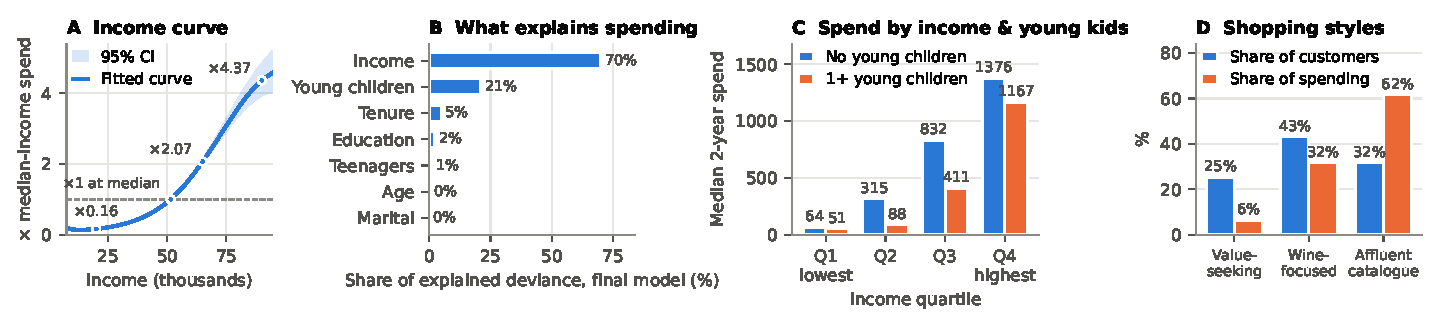
\includegraphics[width=\FigOneWidth]{figures/summary_fig1.pdf}
  \captionof{figure}{(A) Fitted income curve: mean spending relative to a median-income customer, other factors fixed, with 95\% CI. (B) Each factor's share of the final spending model's explanatory power, averaged over every order of adding factors (Shapley decomposition). (C) Median two-year spending by income quartile, with and without young children. (D) Each shopping style's share of customers and of spending. $n = 2{,}026$.}
\end{center}

\q{Q3: Who accepts campaigns?}
\begin{itemize}
  \item Past behaviour is the best guide. Customers who had accepted no earlier campaign accepted the last one 9\% of the time; those who had accepted three or more, 82\% (Fig.~2A).
  \item Comparing otherwise-similar customers, singles are 10 percentage points more likely to accept and PhD holders 7 points more likely, and long-standing customers accept more often too. A teenager at home lowers the chance by 8 points.
\end{itemize}

\begin{center}
  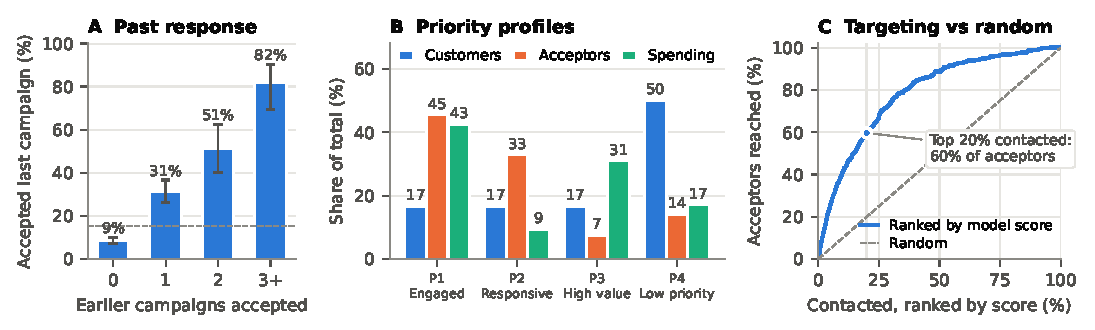
\includegraphics[width=\FigWidth]{figures/summary_fig2.pdf}
  \captionof{figure}{(A) Share accepting the last campaign, by number of earlier campaigns accepted (bars: 95\% confidence intervals; dashed line: 15\% average; $n$ = 1,601/301/74/50). (B) Each profile's share of customers, acceptors and spending. (C) Share of all acceptors found when contacting customers in score order, tested on unseen customers. $n = 2{,}026$.}
\end{center}

\q{Q4: Whom should campaigns focus on?} (Fig.~2B)

{\footnotesize
\begin{tabularx}{\linewidth}{@{}l r r r r X@{}}
\toprule
Profile & Customers & Accepted & Share of acceptors & Share of spending & Suggested action$^{*}$\\
\midrule
P1 Engaged      & 16.7\% & 41.6\% & 45.5\% & 42.6\% & Top priority; lead with wine/meat ranges by catalogue and store\\
P2 Responsive   & 16.6\% & 30.4\% & 32.9\% & 9.3\%  & Cheap web/email offers with a discount\\
P3 High value   & 16.6\% & 6.8\%  & 7.4\%  & 31.0\% & Don't send the usual offer; trial a different one on a small group\\
P4 Low priority & 50.0\% & 4.3\%  & 14.2\% & 17.1\% & No paid outreach; welcome new customers separately\\
\bottomrule
\end{tabularx}\par}
{\footnotesize\itshape $^{*}$Changing the cleaning choices moves no profile share by more than 1.3 points. Suggested actions are ideas to test, not proven effects.\par}

\begin{itemize}
  \item \textbf{Who the P1 customers are.} Compared with the average customer, they are far more likely to have accepted an earlier campaign (66\% vs 21\%), earn more (75k vs 52k), rarely have young children (92\% have none vs 58\%), more often have no teenagers at home (76\% vs 52\%), and have been customers longer (14 vs 12 months). They spend mostly on wine and meat, buy through catalogue and store, and seldom use discounts. \textbf{Customers with these traits should be approached first.}
  \item \textbf{How many to contact.} Contacting the top 20\% of customers by score finds 60\% of all acceptors, and 46\% of those contacted accept; the top 30\% finds 74\% (Fig.~2C).
  \item \textbf{Match the offer to the group.} Campaign 3 was accepted by 21\% of P2 (8\% overall), while P3 accepted every earlier campaign at a below-average rate. Different offers appeal to different customers, so offer content should be tested by profile.
  \item \textbf{What we need from the client:} (1) when the purchase and visit data were recorded; (2) what campaigns 3 and 4 offered; (3) what Z\_CostContact\slash Z\_Revenue mean; (4) a random hold-back group in the next campaign. To detect a 10-point lift it needs about 1,420 targeted customers (210 held back), so it should cover the whole base, not just P1 + P2 (675).
\end{itemize}

% ======================= Challenges | Limitations =======================
\par\vspace{3pt}\noindent
\begin{minipage}[t]{0.485\linewidth}
\section*{Challenges}
We do not know whether purchases and visits were recorded before or after the last campaign, so we left out days since the last purchase. Adding it lifts ranking accuracy (0.5 = random, 1 = perfect) from 0.84 to 0.88, possibly only because of the campaign itself. Duplicates flattered the model (0.839 $\rightarrow$ 0.846), so we removed them. The standard Gamma fit stalled, so we refitted it with a more reliable method.
\end{minipage}\hfill
\begin{minipage}[t]{0.485\linewidth}
\section*{Limitations}
These are associations, not causes: without knowing who received each campaign, ``likely to accept'' is not ``buys because of it''. Behaviour-based scores are optimistic if those data post-date the campaign. Results apply to offers like the last one (acceptance 1--15\% across campaigns) and to 2012--14 customers. Small groups (e.g.\ 19 complainers) give rough estimates, and there are no cost data for profit estimates.
\end{minipage}

\end{document}
